\section{Semi-decidable Predicates}

We have talked primarily about decidable predicates so far. However, in computability theory there are interesting classes of predicates that sit `above' decidable predicates, so to speak. They are `harder` than the decidable predicates because they cannot be computed by a total recursive function, but they still rely on total recursive functions for their definition. 

We will develop a hierarchy of these predicates, starting with the most accessible class, those of \textit{semi-decidable} predicates.

\begin{definition}
A predicate $P(x_1, \ldots x_n) \subseteq \mathbb{N}^N$ is \textit{semi-decidable} if there exists a computable function $c_P^+$, called the positive characteristic function, where \[
    c_P^+(x_1, \ldots x_n) = \begin{cases}
        1 & \text{if } $P(x_1, \ldots x_n)$ \\
        \uparrow & \text{otherwise}
    \end{cases}
\]
\end{definition}

The class of semi-decidable predicates automatically contains every decidable predicate, as a decidable predicate's characteristic function can be forced to loop forever on inputs it excludes.

The primary property of the positive characteristic functions is that they define the predicate by their domain. The definition of the semi-decidable predicate does not depend on the values the characteristic function takes on where it is defined:

\begin{proposition}\label{semidecidable-domain}
An n-ary predicate $P(x_1, \ldots x_n)$ is semi-decidable if and only if it is the domain of some partial recursive $f^{(n)}$.
\end{proposition}
\begin{corollary}
An n-ary predicate $P$ is semi-decidable if and only if there is an $e \in \mathbb{N}$ with $W_e^{(n)} = P$.
\end{corollary}

By this corollary, all semi-decidable predicates can be enumerated by the proper index for a partial recursive function $e$. As $W^{(n)}(e, x_1, \ldots x_n)$ is semi-decidable, it then serves as a `universal' semi-decidable predicate for all semi-decidable n-ary relations, a notion we will define formally later.

There is a strong connection between semi-decidable predicates and partial recursive functions via their graphs. To recall, the graph of a function $f^{(n)}$ is the relation interpreting it as a subset of $\mathbb{N}^{n+1}$: \[
\text{Graph}_f(\overline{x}, y) \iff f(\overline{x}) \downarrow \land \ f(\overline{x}) = y\]

\begin{proposition}\label{graph-decidable}
A partial function $f^{(n)}$ is recursive if and only if  
$\text{Graph}_f(\overline{x}, y)$ is semi-decidable.
\end{proposition}
\begin{proof}
First we show that recursive functions have semi-decidable graphs. Assume that $f$ is a partial recursive function. Then define \[
    c^+_{\text{Graph}_f}(\overline{x}, y) = \begin{cases}
        \overline{\text{sg}}(|f(\overline{x}) - y|) & \text{if } f(\overline{x}) \downarrow \\
        \uparrow & \text{otherwise}
    \end{cases}
\]

$c^+_{\text{Graph}_f}$ halts only if $f$ does, and further outputs 1 only when $\overline{\text{sg}}(|f(\overline{x}) - y|) = 1$, i.e. when $f(\overline{x}) = y$. Therefore it serves as a positive characteristic function witnessing the semi-decidability of $\text{Graph}_f$.

To show that semi-decidable graphs define recursive functions, the idea is to enumerate the possible outputs of the function until the graph tells us we determined the proper one. Due to the semi-decidability of the graph relation, we can only achieve this with a dovetailing strategy.

Let $f$ be a partial function. Let $C_G^+(\overline{x}, y) = \varphi_e$ be the partial recursive positive characteristic function of its graph, with index $e \in \mathbb{N}$. Set

\[
    g^{(n)}(\overline{x}) = \left(\mu z \left[\text{seq}(z) \land \text{lh}(z) = 2 \land T^{(n+1)}(e, \overline{x}, (z)_1, (z)_2)\right]\right)_1
\]
This partial recursive function searches for pairs $z = (y, c)$ with $c$ describing a computation of $\varphi_e(\overline{x}, y)$, returning $y$ when $c$ describes a valid halting computation. Then $g = f$, meaning that $f$ is recursive.
\end{proof}

\Cref{graph-decidable} can give us many useful examples of semi-decidable predicates based on the partial recursive functions. However, the class of semi-decidable predicates is much broader, in the sense that only a few semi-decidable predicates are even valid graphs of functions. The selection theorem gives us a way to produce partial recursive functions from arbitrary semi-decidable predicates, so named because it `selects` a value of the semi-decidable predicate to define for a partial recursive function:

\begin{theorem}{(\textit{Selection})}\label{selection}
If $R^{(n+1)}(\overline{x}, y)$ is a semi-decidable predicate, then there exists a partial recursive $f^{(n)}$ where $f(\overline{x}) \downarrow$ if and only if $\exists y \ R(\overline{x}, y)$, and $R(\overline{x},f(\overline{x}))$ where $f(\overline{x})$ is defined.
\end{theorem}
\begin{proof}
As $R$ is semi-decidable, let $R(\overline{x}, y) \iff \exists z Q(\overline{x}, y, z)$ for decidable $Q^{(n+2)}$. Then define \[
    f(\overline{x}) = \left(\mu s \left[ \text{seq}(s) \land \text{ lh}(s) = 2 \land Q(\overline{x}, (s)_1, (s)_2) \right]\right)_1
\]
This function is partial recursive, and searches for pairs $(y, z)$ such that $Q(\overline{x}, y, z)$. The function only halts upon finding such a pair, which witnesses $R(\overline{x}, y)$.
\end{proof}

The connection between semi-decidable predicates and partial recursive functions established in \Cref{selection} and \Cref{graph-decidable} lets us show properties of partial recursive functions using semi-decidable predicates:
\begin{corollary}\label{partial-inverse}
If $g^{(1)}$ is an partial recursive function, there is a partial recursive $f^{(1)}$ such that $f$ is defined on the range of $g$, and for all $y$ in the range of $g$, $g(f(y)) = y$. Further, if $g$ is injective, then $f = g^{-1}$ for the partial inverse of $g$, so $g^{-1}$ is partial recursive.
\end{corollary}
\begin{proof}
As $g$ is partial recursive, $\text{Graph}_g^{(2)}(x, y)$ is semidecidable. Apply \Cref{selection} to $R^{(2)}(y, x) = \text{Graph}_g^{(2)}(x, y)$ (the graph of $g$ with the arguments swapped) to produce $f$. If $g$ is injective, for any $y$ in the range of $g$ there is only one possible element $x$ such that $g(x) = y$, which $f$ must find by definition.
\end{proof}

Should this come with the picture of the inverse?

It turns out that a more powerful version of \Cref{partial-inverse} is not always true. For a point $y$ in the range of $g$, consider $g^{-1}(\{y\})$, or the set of all points that map to $y$. As \Cref{partial-inverse} provides, $f$ just produces an arbitrary point in $g^{-1}(\{y\})$. If we require $f$ to produce a particular point, i.e. \[
f(y) = \mu x \ \left[ g(x) = y \right]
\] then it is not always recursive.

Semi-decidable predicates are an example of a class `above' decidable predicates in the sense that they also include undecidable predicates. A natural question to ask is if there are classes of predicates `above` semi-decidable predicates. Critically, it turns out that semi-decidable predicates can be written as existentially quantified decidable predicates by the following theorem:

\begin{theorem}\label{defining-sigma1}
A predicate $P^{(n)}(\overline{x})$ is semi-decidable if and only if there is a decidable predicate $Q^{(n+1)}(\overline{x}, y)$ such that for all $\overline{x}$, $P(\overline{x}) \iff \exists y Q(\overline{x}, y)$.
\end{theorem}

\begin{proof}
Assume that $P$ can be written as $\exists y \ Q(\overline{x}, y).$ Then write \[
    c_P^+(x) = \text{const}_1 \left(\mu y \left[Q(\overline{x}, y)\right]\right)
\]

This is the positive characteristic function of $P$, which is partial recursive due to being defined by $\mu$-recursion on the total recursive predicate $Q$.

For the other direction, assume that $P$ is semidecidable. Then by \Cref{semidecidable-domain}, $P$ is the domain of some partial recursive $\varphi_e^{(n+1)}$. Therefore \[P(\overline{x}) \iff \exists z \ T^{(n+1)}(e, \overline{x}, z)\] We are finished because $T$ is a decidable predicate.
\end{proof}

In anticipation of higher classes of predicates that look much like $\exists y \ Q(\overline{x}, y)$, we will give a definition of $\Sigma_1$ predicates:

\begin{definition}
A predicate $P^{(n)}(\overline{x})$ is $\Sigma_1$ if and only if it can be written as $\exists y \ Q(\overline{x}, y)$ for some decidable predicate $Q^{(n+1)}(\overline{x}, y)$.
\end{definition}

As shown by \Cref{defining-sigma1}, the class of semi-decidable predicates is exactly $\Sigma_1$, so they will be used interchangeably from now on.

We might search for harder predicates by composing existing predicates with logical operators. But like decidable predicates, semi-decidable predicates admit some nice closure properties that let us inductively build up more complicated semi-decidable predicates. As the following proposition shows, the characterization of semi-decidable predicates as $\Sigma_1$ lets us prove this fact quite conveniently:

\begin{proposition}\label{semidecidable-closure}
The class of semi-decidable predicates is closed under substitution of partial recursive functions, $\land, \lor$; unbounded quantification $\exists x \leq y$, $\forall x \leq y$; and existential unbounded quantification $\exists x$.
\end{proposition}
\begin{proof}
Closure under substitution of partial recursive functions follows from the closure of partial recursive functions under composition using the positive characteristic function. Closure under $\land$ and $\lor$ can be shown by dovetailing the positive characteristic functions.

To prove closure under quantification, take a semidecidable predicate
$P^{(n+1)}(\overline{x}, z)$, with extra variable $z$ to be removed in the quantified predicates. $P$ is $\Sigma_1$, so can be written as $\exists w \ Q(\overline{x}, z, w)$ for decidable $Q^{(n+2)}(\overline{x}, z, w)$. Then there are three cases for the three forms of closure under quantification:
\begin{enumerate}
    \item Put $R(\overline{x}, y) \iff \exists z \leq y \ P(\overline{x}, z)$. Then \[
        R(\overline{x}, y) \iff \exists z \leq y \ \exists w \ Q(\overline{x}, z, w) \iff \exists w \ \exists z \leq y \ Q(\overline{x}, z, w)\
    \]
    The far-right-hand side is existential quantification over a decidable predicate, so $R$ is semi-decidable.
    \item Put $R(\overline{x}, y) \iff \forall z \leq y \ P(\overline{x}, z)$. Then \[
        R(\overline{x}, y) \iff \forall z \leq y \ \exists w \ Q(\overline{x}, z, w) \iff \exists t \ \forall z \leq y \ \exists w \leq t \ Q(\overline{x}, z, w)
    \]
    $R$ is again an existential quantification over a decidable predicate, so is semi-decidable.
    \item Put $R(\overline{x}) \iff \exists z \ P(\overline{x}, z)$. Then \[
        R(\overline{x}) \iff \exists z \ \exists w \ Q(\overline{x}, z, w) \iff \exists s \ \text{seq}(s)\  \land \text{ lh}(s) = 2 \ \land \ Q(\overline{x}, (s)_1, (s_2))
    \]
    where we replace the double existential search with a single one for pairs, showing $R$ is semi-decidable.
\end{enumerate}
\end{proof}

Many index sets are examples of semi-decidable predicates that are undecidable, which we showed with Rice's theorem. For example, the index set $I(e) \iff \varphi_e^{(1)}(0) \downarrow$ is undecidable, but is semi-decidable due to the closure properties listed above.

\section{The Arithmetical Hierarchy}

In this section, we develop the theory necessary to summarily classify many interesting kinds of predicates in terms of quantifications of decidable predicates, mirroring the definition of $\Sigma_1$ for these `higher' levels.

We can start off by characterizing decidable predicates in terms of semi-decidable ones:

\begin{proposition}\label{delta-1}
A predicate $P^{(n)}(\overline{x})$ is decidable if and only if $P$ and $\lnot P$ are both semi-decidable.
\end{proposition}

\begin{proof}
The forward direction is straightforward: if $P$ is decidable, then it is semi-decidable. $\lnot P$ is also decidable, so it is semi-decidable.
Now assume that $P$ and $\lnot P$ are both semi-decidable. Then $P$ can be written as $\exists z \ Q(\overline{x}, z)$, and $\lnot P$ can be written as $\exists z \ Q^*(\overline{x}, z)$. Then define
\[
    C_P^+(\overline{x}) = \Theta\left(\mu z \left[ Q(\overline{x}, z) \lor Q^*(\overline{x}, z)\right]\right)
\] with \[
    \Theta(z) = \begin{cases}
        1 & \text{if } Q(\overline{x}, z) \\
        \uparrow & \text{otherwise}
    \end{cases}
\]
For a specific input $\overline{x}$, exactly one of $Q$ and $Q^*$ will be satisfied for some $z$. The $\mu$-recursion discovers a $z$ that satisfies either, then $\Theta$ ensures that $C_P^+$ only halts if $Q$ has been satisfied, making it correctly indicate $P$.
\end{proof}

Note that $W^{(n)}(e, \overline{x}) \iff \varphi_e^{(n)}(\overline{x}) \downarrow$ is a semi-decidable predicate, not decidable. If $n=1$, for example, this can be shown because $K(e) \iff W(e, e)$. As a result of this fact and \Cref{delta-1}, we are able to classify several sets and find some examples of predicates that are not semi-decidable:
\begin{corollary}
$\lnot W^{(1)}(e, x)$ is not semi-decidable.
\end{corollary}
\begin{corollary}
$K$ is semi-decidable, $\lnot K$ is not semi-decidable.
\end{corollary}
By classifying $\lnot K$, we can also show that the class of semi-decidable predicates does not satisfy every logical closure property:
\begin{corollary}
The class of semi-decidable predicates is not closed under $\lnot$ or unbounded $\forall x$.
\end{corollary}
\begin{proof}
$K$ is semi-decidable. If the class of semi-decidable predicates was closed under $\lnot$, then $\lnot K$ would be semi-decidable.

Similarly, if the class of semi-decidable predicates was closed under unbounded $\forall x$, then we could show $\lnot K$ was semi-decidable by: \[
    \lnot K(e) \iff \forall x \ \lnot \left(T^{(1)}(e, e, x)\right)
\]
$\lnot \left(T^{(1)}(e, e, x)\right)$ is semi-decidable, so if the entire predicate was semi-decidable, so would be $\lnot K$.
\end{proof}

The fact that the $\Sigma_1$ predicates are not closed unbounded `forall' and negation suggests that it could be useful to examine predicates in terms of their leading quantifiers. We have already seen that predicates of the form \[
    P^{(n)}(\overline{x}) \iff \exists y \ R^{(n+1)}(\overline{x}, y)
\]
where $R^{(n+1)}$ is decidable are semi-decidable. Though $\Sigma_1$ is not closed under negation, we could rewrite predicates that are negations of $\Sigma_1$ predicates in terms of a universal quantifier: \[
    \lnot P^{(n)}(\overline{x}) \iff \lnot \exists y \ R^{(n+1)}(\overline{x}, y) \iff \forall y \ \lnot R^{(n+1)}(\overline{x}, y)
\]
These predicates can be written as a universal quantifier in front of a decidable predicate $R$, and we call such predicates $\Pi_1$. As we have just shown, each predicate in $\Pi_1$ is the negation of a predicate in $\Sigma_1$ and vice versa. By \Cref{delta-1}, the $\Sigma_1$ or $\Pi_1$ predicates that are invariant under negation (in the sense that the complexity of the predicate stays the same under negation) are actually decidable! We can summarize this by denoting all decidable predicates $\Delta_1 = \Sigma_1 \cap \Pi_1$.

The subscripts may hint at the fact that we have even larger similar hierarchies of predicates. Specifically, we have already seen that adding an unbounded universal quantifier can make predicates no longer $\Sigma_1$. Then, such predicates are in the form \[
    P^{(n)}(\overline{x}) \iff \forall y \ \exists z \ R^{(n+1)}(\overline{x}, y, z)
\]
which, following notation already set up, would make sense to be called $\Pi_2$. We will discuss examples of such predicates later on.

$\Pi_2$ has a corresponding negated class $\Sigma_2$, both with corresponding smaller class $\Delta_2 = \Pi_2 \cap \Sigma_2$. Following the intuition set up in \Cref{semidecidable-closure}, we notice that what makes $\Sigma_n$ and $\Pi_n$ predicates `harder' is adding quantifiers of alternating existential and universal type, motivating a full recursive definition of classes we have discussed so far:

\begin{definition}
A predicate $P^{(k)}(\overline{x})$ is in $\Sigma_n$ if it can be written as $n$ alternating unbounded quantifiers, starting with an $\exists$, in front of a decidable predicate $Q^{(n+k)}$: \[
    P(\overline{x}) \iff \exists y_1 \ \forall y_2 \ \ldots y_n \ Q(x_1, \ldots x_k, y_1, \ldots y_n)
\]
$P$ is in $\Pi_n$ if it can be written as $n$ alternating unbounded quantifiers that start with a $\forall$:
\[
    P(\overline{x}) \iff \forall y_1 \ \exists y_2 \ \ldots y_n \ Q(x_1, \ldots x_k, y_1, \ldots y_n)
\]
$P$ is in $\Delta_n$ if it is both in $\Pi_n$ and $\Sigma_n$.
\end{definition}

These definitions can be summarized with \Cref{hierarchy-figure}, with previously-discussed predicates $K$ and $\lnot K$ marked with their proper places in the diagram.

\begin{figure}[H]
\centering
    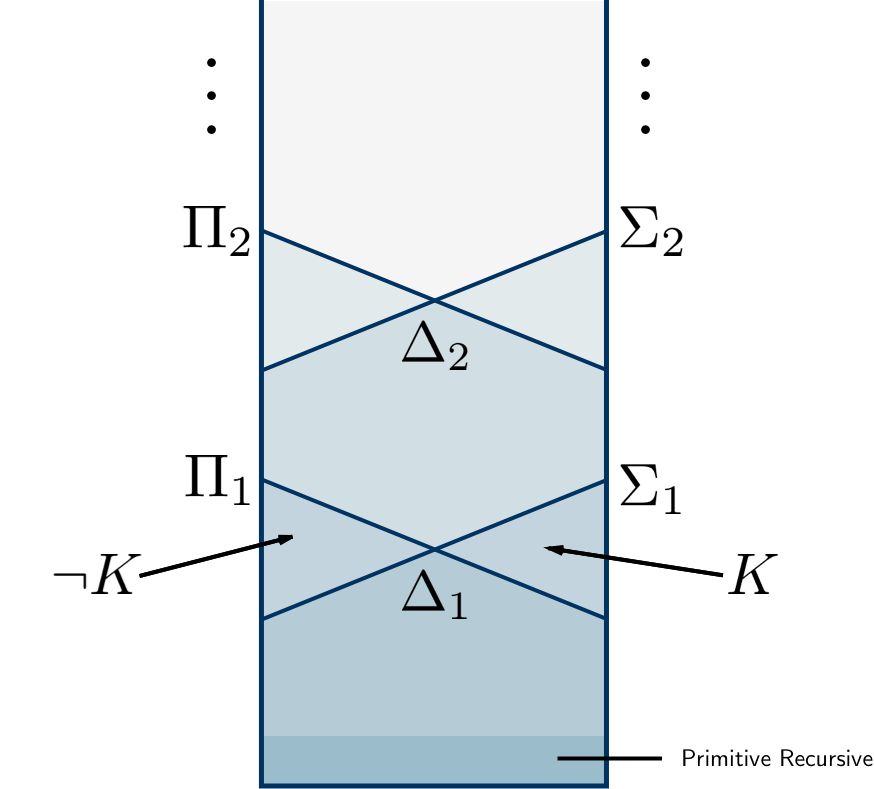
\includegraphics[height=3in]{figs/arithmetical-hierarchy.png}
\caption{A diagram of the arithmetical hierarchy}
\label{hierarchy-figure}
\end{figure}

We have shown that the class of primitive recursive predicates is strictly smaller than $\Delta_1$, and so they belong towards the bottom of the hierarchy. It is interesting to note that most of the classes examined in computational complexity theory, \textsc{P}, \textsc{NP}, \textsc{PSPACE} and the like, are strict subsets of $\Delta_1$ as it is possible to decide their predicates by computer (regardless of how long the decision takes). In this course we don't particularly care about the efficiency of our algorithms, just about their existence; such efficiency considerations are discussed in CS 170.

Placing certain sets in this hierarchy is not always straightforward. In addition, so far to `lower bound' sets like $K$ and $\lnot K$, excluding them from $\Delta_1$, we have used techniques that do not easily generalize. We will examine some ways to bound predicates via universality, many-to-one reductions, and completeness.

\begin{definition}
A predicate $V^{(n+1)}(e, x_1, \ldots x_n)$ is $\Sigma_1$\textit{-universal} if
\begin{enumerate}
    \item $V$ itself is $\Sigma_1$.
    \item For any n-ary $\Sigma_1$ predicate $P^{(n)}(\overline{x})$, $P$ is a subsection of $V$, i.e. there is an index $e$ where for all $\overline{x}$, $P(\overline{x}) \iff V(e, \overline{x})$. Here we say $P = V_e^{(1)}$.
\end{enumerate}
\end{definition}

We have already seen an example in the form of $W^{(n+1)}(e, x_1, \ldots x_n) \iff \varphi_e(x_1, \ldots x_n) \downarrow$, whose index $e$ ranges through the domains of all $n$-ary $\Sigma_1$ predicates.

Here we have a lower bound, as no $\Sigma_1$-universal sets can be $\Pi_1$, excluding them from $\Delta_1$. We prove it for the $n=1$ case:

\begin{proposition}
If $V^{(2)}(e, x)$ is $\Sigma_1$-universal, then it is not $\Pi_1$.
\end{proposition}
\begin{proof}
Assume $V$ is $\Pi_1$. Consider the set $S^{(1)}(e) \iff V^{(2)}(e, e)$. As $S$ is $\Pi_1$, $\lnot S$ is $\Sigma_1$, so $\lnot S$ must have some index $f$ where $\lnot S = V_f^{(1)}$. But then \[
\lnot S(f) \iff V^{(2)}(f,f) \iff S(f)
\]
which is a contradiction.
\end{proof}

$\Sigma_1$-universal predicates are quite powerful, but are too strong for many predicates strictly in $\Sigma_1$. We can adapt the technique of many-to-one reduction introduced earlier in the related notion of $\Sigma_1$-complete sets. Note that here we only interpret $\Sigma_1$ predicates as subsets of $\mathbb{N}$, which can be done systematically for $n$-ary predicates using the sequence coding.

\begin{definition}
A set $V \subseteq \mathbb{N}$ is $\Sigma_1$\textit{-complete} if $V$ is $\Sigma_1$, and for all $\Sigma_1$ sets $B \subseteq \mathbb{N}$ we have that $B \leq_m V$.
\end{definition}

We can connect the two notions by a way to generate $\Sigma_1$-complete sets related to $\Sigma_1$-universal sets.

\begin{proposition}\label{producing-sigma-1-complete}
Let $V^{(n+1)}(e, x_1, \ldots x_n)$ be $\Sigma_1$-universal. Let \[
V^*(s) \iff \text{seq}(s) \land \text{ lh}(s) = n+1 \land V^{(n+1)}((k)_1, \ldots, (k)_n, (k)_{n+1})
\]
Then $V^*$ is $\Sigma_1$-complete.
\end{proposition}

If we apply \Cref{producing-sigma-1-complete} to $W^{(2)}(e, x)$, we produce the $\Sigma_1$-complete $W^*(n)$, which tells us if $\varphi_{(n)_1}\left((n)_2\right) \downarrow$, i.e. the general halting problem as a subset of $\mathbb{N}$. This suggests that $K$ is $\Sigma_1$-complete despite seeming less powerful, which is in fact true!

\begin{proposition}
K is $\Sigma_1$-complete.
\end{proposition}
\begin{proof}
We have already shown that $K$ is $\Sigma_1$. Now let $B \subseteq \mathbb{N}$ be $\Sigma_1$. To perform the many-to-one reduction and show $B \leq_m K$, we are looking for a total recursive $t$ such that $B(e) \iff K(t(e))$.

By S-m-n, we arrange $\varphi_{t(e)}(x) = c_B^+(e)$ via partial recursive $f(e, x) = c_B^+(e)$. Then $K(t(e)) \iff \varphi_{t(e)}(e) \downarrow \iff c_B^+(e) \downarrow \iff B(e)$ as desired.
\end{proof}
The transitivity of $\leq_m$ leads to a nice shortcut to proving that sets are $\Sigma_1$-complete via only one many-to-one reduction.
\begin{proposition}
Let $S \subseteq \mathbb{N}$ be $\Sigma_1$. If $K \leq_m S$, $S$ is $\Sigma_1$-complete.
\end{proposition}

Informally, by showing $A \leq_m B$ for some sets $A$ and $B$, we determine that $B$ is `at least as hard' as $A$ on the arithmetical hierarchy, and perhaps `harder'. Then the $\Sigma_1$-complete sets belong at the `top tip' of $\Sigma_1$, as they are at least as high as all sets in $\Sigma_1$. This provides some nice bounds on where these sets lie in the arithmetical hierarchy.

We can expand the class of $\Sigma_1$-complete sets further to include many index sets using what is a corollary to Rice's theorem.

\begin{proposition}\label{index-set-complete}
Let $I$ be a nontrivial $\Sigma_1$ index set. Then $I$ is $\Sigma_1$-complete.
\end{proposition}
\begin{proof}
Via Rice's theorem, we showed that $K \leq_m I$ or $K \leq_m \overline{I}$. But $\overline{I}$ is $\Pi_1$ by definition, so if $K \leq_m \overline{I}$, $K$ is $\Pi_1$, which is a contradiction.
\end{proof}

Here are several examples of sets we now know to be $\Sigma_1$-complete:
\begin{enumerate}
    \item $I(e) \iff \varphi_e(0) = 0$
    \item $I(e) \iff \exists x \ x \text{ even} \land \varphi_e(x) \downarrow$
    \item $I(e) \iff \varphi_e(0) = 0 \land \exists y \ \varphi_e(y) \text{ even}$
\end{enumerate}

The index set $\text{Tot}(e) \iff \left(\varphi_e^{(1)} \text{ total}\right)$ has the property that all $\Sigma_1$ sets reduce to it, but it is not $\Sigma_1$-complete, as it is too hard to be in $\Sigma_1$. 

\section{Characterizing $\Sigma_1$ Index Sets}
We have already shown that $\Sigma_1$ index sets are $\Sigma_1$-complete by \Cref{index-set-complete}. In this section, we aim for a much stronger characterization of the $\Sigma_1$ index sets that reveals a surprising structure that respects the natural order of functions. We will also use similar ideas later on when discussing the Recursion theorems.

Our definition of partial functions from $\mathbb{N} \rightarrow \mathbb{N}$ as sets admits a partial order defined in terms of $\subseteq$, or function extension. The empty function $\varnothing$ is a subset of all functions, and serves as a unique `least element' of this order. As a basis for all partial recursive functions, we first examine finite functions, or functions defined on a finite subset of $\mathbb{N}$.
\begin{definition}
A natural number $b$ codes a finite function if \begin{enumerate}
    \item $\text{seq}(b)$ and $\forall k \leq \text{lh}(b) \ \text{seq}\left( (b)_k \right) \land \text{lh}\left((b)_k\right) = 2$
    \item $\forall k, j \leq \text{lh}(b) \ ((b)_k)_1 = ((b)_j)_1 \implies ((b)_k)_2 = ((b)_j)_2$
\end{enumerate}
\end{definition}
This definition essentially describes graphs of finite functions, encoded as sequences of pairs $(x, f(x))$. The second property ensures that the graph is a function that assigns at most one value to each point in the domain. The predicate $\text{Fn}(b)$ defined by these two conditions is primitive recursive. As a notational convenience, we use the notation $f_b$ to denote the finite function coded by b:
\begin{definition}
If $\text{Fn}(b)$, then $f_b$ is the function that $b$ codes. In other words, $a \in \text{dom}(f_b)$ if and only if $\exists k \leq \text{lh}(b) \ ((b)_k)_1 = a$; and for such $a$, $f_b(a) = c$ if and only if  $\exists k \leq \text{lh}(b) \ ((b)_k)_1 = a \land ((b)_k)_2 = c$.
\end{definition}
This coding of finite functions by natural numbers admits an effective way to convert codes to an index of the equivalent partial 1-ary function.
\begin{lemma}
There is a total recursive function $t$ such that for all $b$, $\text{Fn}(b) \implies \varphi_{t(b)}^{(1)} = f_b$, and $\lnot \text{Fn}(b) \implies \varphi_{t(b)}^{(1)} = \varnothing$.
\end{lemma}
\begin{proof}
Define \[
    g(b, x) = \begin{cases}
        f_b(x) & \text{if } \text{Fn}(b) \land x \in \text{dom}(f_b) \\
        \uparrow & \text{otherwise}
    \end{cases}
\]
$g$ is partial recursive, and by S-m-n we produce the required $t$.
\end{proof}
Note that there is no partial recursive function that performs the inverse, i.e. $h$ such that $f_{h(e)} = \varphi_e^{1}$, defined only on e for which $\text{dom}(\varphi_e^{(1)})$ is finite.
\section{Recursively Enumerable Sets}
\section{Simple Sets}
\section{Hypersimple Sets}
